
%%%%%%%%%%%%%%%%%%%%%%%%%ll19_prlv1.tex%%%%%%%%%%%%%%%%%%%%%%%%%%%%%%%%%%%%

\documentclass[aps,nofootinbib,prl,showpacs,twocolumn,groupedaddress,superscriptaddress]
{revtex4}
\usepackage{graphicx} 
\usepackage{dcolumn} 
\usepackage{longtable} 
\usepackage{amssymb} 
\usepackage{bbold}
\usepackage{amsmath} 
\usepackage{amsfonts} 
\usepackage{slashed} 
\usepackage[dvipsnames]{xcolor} 
\usepackage{soul}
%=============================================================================
\newcommand*{\mprime}{^{\prime}\mkern-1.2mu}
\newcommand*{\mdprime}{^{\prime\prime}\mkern-1.2mu}
\newcommand*{\mtprime}{^{\prime\prime\prime}\mkern-1.2mu}
\newcommand{\red}[1]{\textcolor{red}{#1}}
\newcommand{\green}[1]{\textcolor{green}{#1}} 
\newcommand{\gray}[1]{\textcolor{gray}{#1}} 
\newcommand{\blue}[1]{\textcolor{blue}{#1}} 
\newcommand{\bs}[1]{\boldsymbol{#1}} 
\newcommand{\nopieft}{\mbox{$\slashed{\pi}$EFT}} 
\newcommand{\eftnopi}{\mbox{EFT($\slashed{\pi}$) }} 
\newcommand{\Lag}{{\cal L}} 
\newcommand{\be}{\begin{equation}} 
\newcommand{\ee}{\end{equation}} 
\newcommand{\rvec}{{\bs{r}}} 
\newcommand{\xvec}{{\bs{x}}} 
\newcommand{\sgmvec}{\ensuremath{\boldsymbol{\sigma}}} 
\newcommand{\tauvec}{\ensuremath{\boldsymbol{\tau}}} 
\newcommand{\half}{\frac{1}{2}}
\newcommand{\eg}{\textit{e.g.}\;}
\newcommand{\ie}{\textit{i.e.}\;}
\newcommand{\etc}{\textit{etc.}\;}
\newcommand{\ve}[1]{\ensuremath{\boldsymbol{#1}}}
\newcommand{\ddrei}[1]{\delta_{\tiny \Lambda}^{(3)}\!\big(#1\big)}
%=============================================================================

\begin{document}

\title{-TBD-} 


\title{JLM-Machester}
\author{J K L C M S}


\date{\today}

\begin{abstract}
We present the first comprehensive study of few identical bosons and bosonic-fermionic mixture in function of the two body scattering length $a_0$, effective range $r_0$ and thrre-bosons binding energy $B_3$.
Employing a spin-independent interaction among all the particles, we show the existence of a minimum effective range $\bar{r}_0$ required to support bound states in 2-fermions n-bosons systems ($F(2)B(n)$ and $F_1(2)F_2(2)B(n)$).
$\bar{r}_0$ results to be always finite and dependent both from the number of bosons in S-shell and the ratio between two and three-body Efimov scales ($a_0 B_3$).
 
This study has several implications not only in atomic physics, where the interaction between $He$ atoms is fined tuned close to unitarity, but also in nuclear physics where it proofs that a contact interaction can not effectively describe a P-wave bound systems (E.g. $^6$He).
\end{abstract}

\maketitle

\section{Introduction}

The stability of a mixture of ${}^{40}$K fermions and ${}^{87}$Rb bosons\footnote{In the remainder, $B_{n_B}F_{n_F}$ refers to a system of $n_B$ distinguishable
bosons and $n_F$ indistinguishable (fermi) particles.} is known to depend on the number of atoms in the system
(experiment:~\cite{Modugno2240} and theoretical analysis:~\cite{PhysRevA.68.043626}). An analogous nuclear behavior is suggestive, as the atomic
scattering lengths, $a_{BB}\sim-20\,$nm and $a_{BF}\sim 5.2\,$nm, have the ration as the singlet and triplet nucleon-nucleon counterparts, respectively.

\paragraph{The contact theory and examples}
All systems whose constituent's de Broglie wavelength $\lambda$ is
\paragraph{Known limitations of this EFT}
cluster theory for 3/2 resonance needs eff range,
bosonic atoms, 
16O, 
nuclear pectrum, 
\paragraph{The universal system}
A momentum-independent zero-range theory does not predict key features of these exemplary systems.
These features, \eg, stable bound states,
are related to wave functions of mixed spatial symmetry.
This is a consequence of the number of particles,
which is larger than the number of internally accessible degrees of freedom for all the given examples.
Therefore, the internal ((iso)spin, flavour, colour, \etc)
state is of mixed symmetry which implies the same for the spatial component,
because both must combine to a totally anti-symmetric wave function for indistinguishable particles.

description of ABCD..Z, 
Why we use e3=3/4 etch... 
how ABABCD is telated to 6Li, 
neutrons - nuclei - quarks - Lnnn - pnnn.
State mass. (malik)


do we need r0>0 at LO?
or P-wave?

\section{theory and methods}
Pionless - regulator - effective range - fitting, 
cut-off behaviour, 
SVM, 

\paragraph{effective range behaviour}
In \cite{Phillips} was demostrated that the effective range of a square well is 

\begin{equation}
    r_0 = 2 [R-\frac{R^2}{a}+\frac{R^3}{3 a^2}]
\end{equation}

where $R$ is the range of the square well. We expect similar result where the range of the gaussian is $1/\lambda$:

\begin{equation}
    \frac{r_0}{a} = \frac{ \alpha}{\lambda a}+ \frac{\beta}{(\lambda a)^2}+ \frac{\gamma}{(\lambda a)^3}.
    \label{eq:philips_effr}
\end{equation}



\begin{figure}[htb] 
\begin{center} 
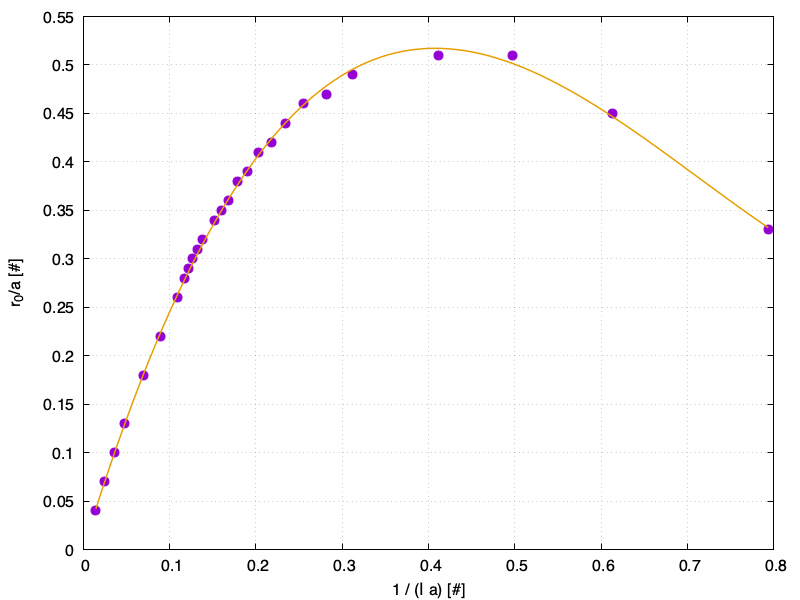
\includegraphics[width=0.4\textwidth]{Graf/effective_range.png}
\caption{Effective range behaviour with respect to the cut-off $\lambda$. The parameters $\alpha$, $\beta$, and $\gamma$ in equation \ref{eq:philips_effr} are respectively 2.9, -5.0, and 2.4 . those number are of order $\sim 1$ as expected.}
\label{fig:fig1}
\end{center} 
\end{figure}

\paragraph{The inter-cluster potential}
In order to study the large-$N$ limit, we develop a model inspired by the resonating-group formalism
(\cite{Wheeler:1937zz},\cite{Wildermuth1977s}).
That entails the assumption of a frozen $A$-body core whose spatially symmetric wave function we
parametrize with a single parameter $a$ via
\be\label{eq.rgm.corewfkt}
\phi_A:=e^{-\frac{a}{2}\sum_{i=1}^A\left(\ve{r}_i-\ve{R}_A\right)^2}\;\;\;;
\begin{array}{l}
     \ve{r}_i\;\;\text{\scriptsize : single-particle coordinates}  \\
     \ve{R}_A\;\;\text{\scriptsize : core centre of mass}
\end{array}\;\;.
\ee
The system is thereby reduced to only three degrees of freedom, namely the relative distance
between core and the odd particle. The respective equation of motion reads in terms of the effective
mass $\mu$, the relative kinetic energy $E$ between core and odd particle:
\be\label{eq.rgm.eqom}
\int\left\lbrace~\phi^*_A\left(-\frac{\hbar}{2\mu}\ve{\nabla}_R^2-E+\mathcal{V}_{A,A+1}\right)
\mathcal{A}\left[\phi_A\psi(\ve{R})\right]\right\rbrace d\ve{r}_{1\ldots A}=0\;\;.
\ee
Antisymmetrization is required between two particles only, $\mathcal{A}=\mathbb{1}-P_{A,A+1}$, and the
interaction term is given by
\begin{align}
\mathcal{V}_{A,A+1}=&~C_0(\Lambda)\sum_{i<j}^X\ddrei{\ve{r}_i-\ve{r}_j}\\
&+D_1(\Lambda)\sum^X_{i<j<k\atop\text{\tiny cyclic}}\ddrei{\ve{r}_i-\ve{r}_j}\,
\ddrei{\ve{r}_j-\ve{r}_k}\;\;.\nonumber
\end{align}
The integration in \eqref{eq.rgm.eqom} yields a three-dimensional Schr\"odinger equation with a
non-local potential
\begin{widetext}
\be\label{eq.rgm.sglnonloc}
\left(\ve{\nabla}_R^2-E\right)\psi(\ve{R})=\sum_{n=1}^3\eta_n~e^{-\kappa_n\ve{R}^2}\psi(\ve{R})+
\sum_{n=1}^4\zeta_n\int\left\lbrace\mathcal{O}_ne^{-\alpha_n\ve{R}^2-\beta_n\ve{R}\cdot\ve{R}'
-\gamma_n\ve{R}'^2}\right\rbrace\psi(\ve{R}') d\ve{R}'\;\;.
\ee
\end{widetext}
The coefficients $\alpha,\ldots,\kappa$ are functions of the number of core particles $A$,
the core size $a$, the interaction regulator $\Lambda$, and the single-particle mass $m$,
and $\mathcal{O}_1=\ve{\nabla}_R^2$, while $\mathcal{O}_{2,3,4}=\mathbb{1}$.

A few comments are in order. Firstly, $\zeta_{1\ldots4}=0$ if $\mathcal{A}=\mathbb{1}$, \ie, the
inter-cluster potential is local. The first non-local term encodes the so-called exchange interaction.
It is non-zero even in the absence of inter-particle forces. The two- and three-body
contact forces affect the inter-cluster potential structurally in the same way. However, the respective
coefficients differ significantly in their dependence on $A,a$ and $\Lambda$. It is the combination
of both, the two- and three-body terms, which results in the changing character of the interaction,
the formation of attractive and repulsive regions, and thereby the possibility to bind the odd particle
to the core. We postpone a detailed analysis of the sensitivity of the inter-cluster potential,
for now, and continue with the discussion of the emerging spectrum of \eqref{eq.rgm.sglnonloc}.

The latter we obtain, again, via the SVM.
\section{results}

Graphics P-wave binding, 
say what is L* and that depend on N, 
the analytical form will benchmark it.

Graphics L* vs N, 
analytical go beyond and tell us what happens.

L* increases with E3/E2,
Unitary limit (is or not bound if a2 -> inf? ).
why a finite L* where it is?

not analyzed mass dependence. (can we do it in analytical bla.bla.)

\paragraph{Stabilization correlated with 2-body interaction details}
We found the stability of the

\subsection{Nuclear case}

Nuclear graphics. 
From 6Li to 8Be, 
Order of states of P-wave, 
to oxygen, 
correct decay modes, 
L*(8Be) < L*(6Li)

\section{Discussion and conclusion}

Stabilization mechanism r0 vs a1, 
perturbative pole motion ?

\section{to do:}
a1 vs r0

N -> inf

mass -> inf

\begin{figure}[htb] 
\begin{center} 
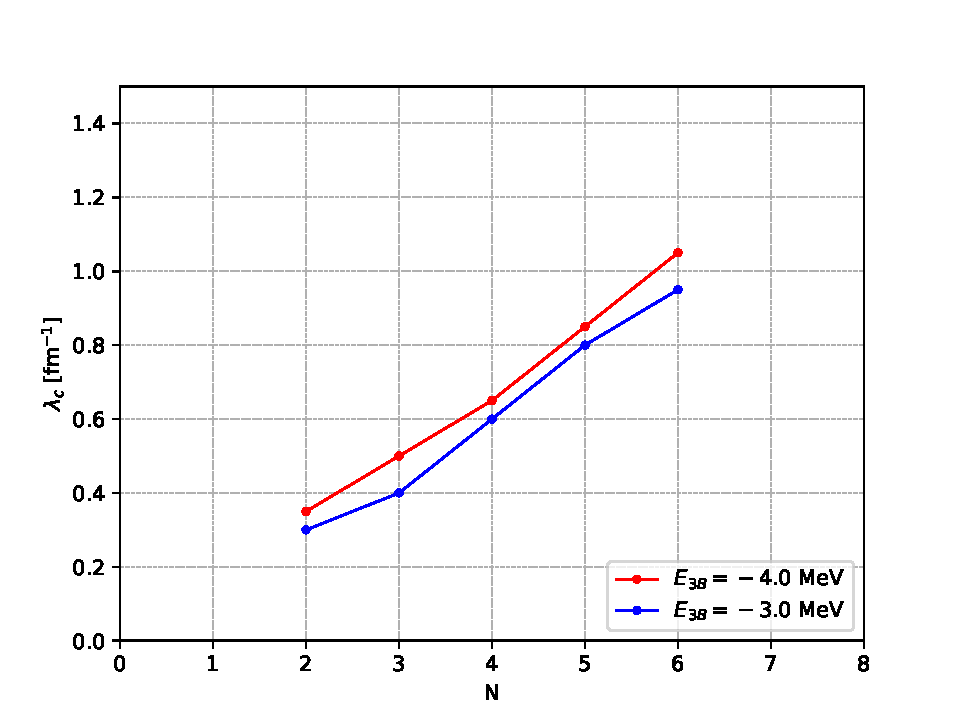
\includegraphics[width=0.4\textwidth]{Graf/Lc-vs-N.pdf}
\caption{}
\label{fig:fig1}
\end{center} 
\end{figure}

\begin{figure}[htb] 
\begin{center} 
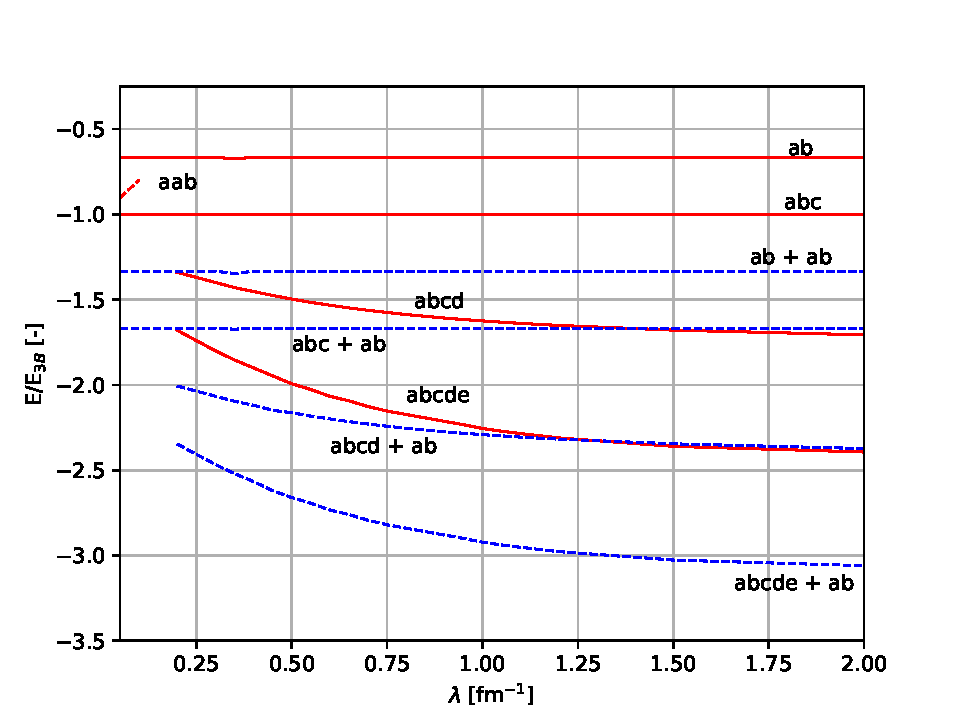
\includegraphics[width=0.4\textwidth]{Graf/E3b15-thresholds.pdf}
\caption{}
\label{fig:fig2}
\end{center} 
\end{figure}

\newpage

\begin{widetext}
\begin{turnpage}
\section{Appendix: Inter-cluster Potential}
\begin{table}
\setlength{\tabcolsep}{4pt}
\renewcommand{\arraystretch}{2.4}
\caption{\label{tab.rgmpot}{Defining parameters of the effective potential between
a Gaussian $A$-body core, characterized via the width $a$~\eqref{eq.rgm.corewfkt},
and one {\it odd} particle (see \eqref{eq.rgm.sglnonloc}).
The 2- and 3-body LECs $C^\Lambda_0$ and $D^\Lambda_1$ are
calibrated to a 2- and 3-body symmetric bound state (see table~\ref{tab.legend}). $A\mprime=A-1$, and
$\mathcal{O}_1=\ve{\nabla}_R^2$, while $\mathcal{O}_{2,3,4}=\mathbb{1}$.}}
\small\centering
\begin{tabular}{lc|ccc}
\hline\hline
$i$ & $\eta_i$ & $\kappa_i$ & & \\
1   & $8~C_0^\Lambda~\frac{A\mprime}{\left(4+\frac{A\mprime}{A}\frac{\Lambda^2}{a}\right)^{3/2}}$  & $\frac{A\Lambda^2}{4A+A\mprime\frac{\Lambda^2}{a}}$ \\
2   & $
\frac{32 D_1^\Lambda a^3 A\mdprime A\mprime}{\left(16 a^2 A+4 a (3 A-1) \Lambda ^2+A\mdprime \Lambda ^4\right)^{3/2}}$ & $\frac{\Lambda ^2 \left(4 a^2 A+2 a A \Lambda ^2\right)}{16 a^2 A+4 a (3 A\mdprime+5) \Lambda ^2+A\mdprime \Lambda ^4}$ \\
3 & 
$\frac{32 D_1^\Lambda A\mdprime A\mprime}{\left(\frac{\left(4 a+\Lambda ^2\right) \left(4 a A+A\mdprime \Lambda ^2\right)}{a^2 A}\right)^{3/2}}$ & $\frac{2 a A \Lambda ^2}{4 a A+A\mdprime \Lambda ^2}$ \\
\hline
$n$ & $\zeta_i$ & $\alpha_n$ & $\beta_n$ & $\gamma_n$ \\
1 &$\frac{2 \sqrt{2}}{\left(\frac{A\mprime (A+1)^2}{a A^3}\right)^{3/2}}$&
$\frac{a \left(A^3+A\right)}{2 A\mprime (A+1)^2}$&
$\frac{2 a A^2}{A\mprime (A+1)^2}$&
$\frac{a \left(A^3+A\right)}{2 A\mprime (A+1)^2}$\\
2 & 
$ \frac{8 C_0^\Lambda a^3 A\mprime A^{9/2}}{\pi ^{3/2} (A+1)^3 \left(4 a A\mprime+A\mdprime \Lambda ^2\right)^{3/2}}  $ & 
$\frac{\text{} a A \left(4 a \left(A^2+1\right)+\left(3 A^2+A+2\right) \Lambda ^2\right)}{2 (A+1)^2 \left(4 a A\mprime+A\mdprime \Lambda ^2\right)}$&
$\frac{4 \text{} a A^2 \left(2 a+\Lambda ^2\right)}{(A+1)^2 \left(4 a A\mprime+A\mdprime \Lambda ^2\right)}$&
$\frac{a A \left(4 a \left(A^2+1\right)+\left(A^2-A+2\right) \Lambda ^2\right)}{2 (A+1)^2 \left(4 a A\mprime+A\mdprime \Lambda ^2\right)}$ \\
3 &
$\frac{32 D_1^\Lambda A\mdprime A\mprime (a A)^{9/2}}{\pi ^{3/2} (A+1)^3 \left(16 a^2 A\mprime+4 a (3 A-4) \Lambda ^2+A\mtprime \Lambda ^4\right)^{3/2}}$&
$\frac{\text{} a A \left(16 a^2 \left(A^2+1\right)+4 a \left(5 A^2+A+4\right) \Lambda ^2+\left(5 A^2+2 A+3\right) \Lambda ^4\right)}{2 (A+1)^2 \left(16 a^2 A\mprime+4 a (3 A-4) \Lambda ^2+A\mtprime \Lambda ^4\right)}$&
$\frac{2 \text{} a A^2 \left(16 a^2+16 a \Lambda ^2+3 \Lambda ^4\right)}{(A+1)^2 \left(16 a^2 A\mprime+4 a (3 A-4) \Lambda ^2+A\mtprime \Lambda ^4\right)}$&
$\frac{a A \left(16 a^2 \left(A^2+1\right)+4 a \left(3 A^2-A+4\right) \Lambda ^2+\left(A^2-2 A+3\right) \Lambda ^4\right)}{2 (A+1)^2 \left(16 a^2 A\mprime+4 a (3 A-4) \Lambda ^2+A\mtprime \Lambda ^4\right)}$\\ 
4 &
$\frac{32 D_1^\Lambda A\mdprime A\mprime}{\pi ^{3/2} \left(\frac{(A+1)^2 \left(4 a+\Lambda ^2\right) \left(4 a A\mprime+A\mtprime \Lambda ^2\right)}{a^3 A^3}\right)^{3/2}}$&
$\frac{\text{} a A \left(4 a \left(A^2+1\right)+\left(5 A^2+2 A+3\right) \Lambda ^2\right)}{2 (A+1)^2 \left(4 a A\mprime+A\mtprime \Lambda ^2\right)}$&
$\frac{2 \text{} a A^2 \left(4 a+3 \Lambda ^2\right)}{(A+1)^2 \left(4 a A\mprime+A\mtprime \Lambda ^2\right)}$&
$\frac{a A \left(4 a \left(A^2+1\right)+\left(A^2-2 A+3\right) \Lambda ^2\right)}{2 (A+1)^2 \left(4 a A\mprime+A\mtprime \Lambda ^2\right)}$\\
\end{tabular}
\end{table}
\end{turnpage}
\end{widetext}
\newpage

\section{Appendix: breaking scales}

The breaking scale of the theory of a given p-wave system of A+1 particles is the smallest scale present in the system, however, the cut-off used to extrapolate results should be chosen to be at least of the order of the hardest scale, usually given by the binding of the first symmetric subsystem.
The momentum scales of each system are the two-body scattering length which is unnaturally large $\aleph = 1/a$ and the many body momentum of each subsystem $M_n=\sqrt{m_N \frac{B_n}{n}}$ with $n\le A$ the number of particle in the system.
In essence, since $\aleph$ is usually the softer scale and $M_n$ with $n=A$ id the harder soft-scale which fixes the minimal reasonable cut off of the theory.
In table \ref{Tab:scales} are listed the breaking scales and the critical $\lambda$ for different systems.

\begin{center}
\begin{tabular}{ |c|c c | c c | c c | c c | c c | c c | } 
 \hline
System           & $\aleph$ & $\lambda_c^{1+1}$ & $M_2$ & $\lambda_c^{2+1}$ & $M_3$ & $\lambda_c^{3+1}$ & $M_4$ & $\lambda_c^{4+1}$ & $M_5$ & $\lambda_c^{5+1}$ & $M_6$& $\lambda_c^{6+1}$  \\ 
$E_3=3$, $E_2=1$  & 0.15 &    - & 0.11 & 0.3    & 0.16 & 0.4 & 0.20 & 0.60 & 0.22 & 0.8 & 0.23 & -\\
$E_3=4$, $E_2=1$  & 0.15 & 0.16 & 0.11 & 0.3    & 0.18& 0.50 & 0.23 & 0.65 & 0.27 & 0.8 & 0.29&1.05\\ 
$E_3=1.5$, $E_2=1$& 0.15&-&0.11&-&0.09&-&0.12&-&0.11&-&-&-\\
Nuclear           & 0.22&-&0.16&0.55&0.26&0.75&0.34&0.95&-&-&-&-\\
$E_3=1$, $E_2=0$  & 0&-&0&0.1&0.09&0.5&0.16&0.7&0.20&0.8&0.23&-\\
 \hline
\end{tabular}
\end{center}

\bibliographystyle{unsrt}
\bibliography{Thebibliography.bib}
\end{document}
